\subsection{ESP32-C6-DEV-KIT-N8 als zentrale Steuereinheit}
Das ESP32-C6-DEV-KIT-N8 (vgl. Abb.~\ref{fig:ESP32C6}) von Waveshare stellt eine kompakte und vielseitige Entwicklungsplattform für eingebettete Systeme dar. 

\begin{figure}[H]
	\centering
	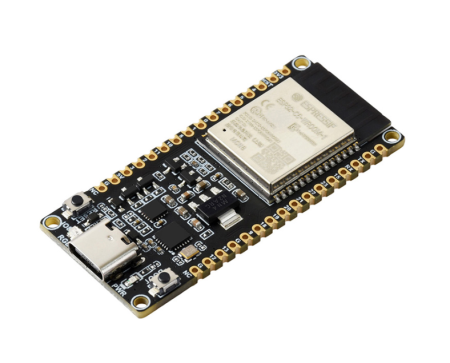
\includegraphics[width=0.5\linewidth]{inhalt/bilder/ESP32-C6-DEV-KIT-N8.png}
	\caption{Waveshare ESP32-C6-DEV-KIT-N8~\cite{WaveshareESP32C6}.}
    \label{fig:ESP32C6}
\end{figure}

Es basiert auf dem \gls{esp32c6} und ist für Anwendungen im Bereich des \gls{iot} ausgelegt. 
Das System unterstützt drahtlose Kommunikation über \gls{wlan} sowie \gls{ble}~\cite{WaveshareESP32C6}. 
Mit der integrierten \gls{wlan}-Schnittstelle ist eine flexible Integration in vernetzte Anwendungen möglich und der \gls{esp32c6} kann als eigenständiges System betrieben werden. 
Er ermöglicht sowohl die Erfassung als auch die Verarbeitung und Übertragung von Daten direkt auf dem Gerät. 
Durch diese Eigenschaften eignet er sich insbesondere für kostengünstige und skalierbare Anwendungen im Bereich vernetzter Systeme~\cite{hernandez2022wifi}.

Ein weiterer Vorteil moderner \gls{wlan}-fähiger Mikrocontroller liegt in der Möglichkeit, Daten direkt auf dem Gerät zu verarbeiten. 
Dadurch können Funktionen wie Analyse oder Entscheidungsfindung lokal umgesetzt werden, ohne auf externe Systeme angewiesen zu sein. 
Dieser Ansatz reduziert die Abhängigkeit von zentralen Recheneinheiten und ermöglicht eine dezentrale Systemarchitektur~\cite{hernandez2022wifi}.

Der \gls{esp32c6} unterstützt weiterhin die Funkstandards Thread und Zigbee. 
Beide Protokolle basieren auf dem \gls{ieee802154}-Standard und sind für energieeffiziente drahtlose Kommunikationssysteme im \gls{iot} ausgelegt.
Durch diese Unterstützung eignet sich der Mikrocontroller insbesondere für Anwendungen im Smart-Home-Umfeld sowie für vernetzte Sensorsysteme mit geringem Energieverbrauch~\cite{WaveshareESP32C6}.
Das Entwicklungsboard verfügt über eine Vielzahl von digitalen Ein- und Ausgängen, die für die Ansteuerung externer Komponenten genutzt werden können (vgl. Abb.~\ref{fig:ESP32C6Pinout}). 

\begin{figure}[H]
	\centering
	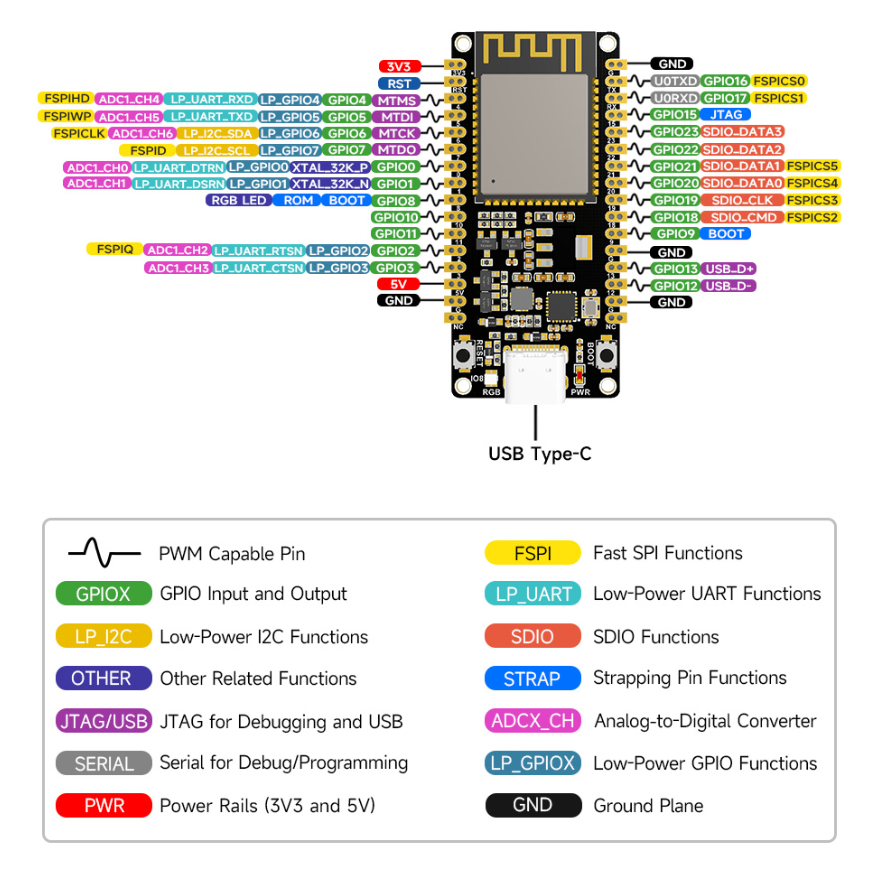
\includegraphics[width=0.7\linewidth]{inhalt/bilder/ESP32-C6-DEV-KIT-N8_Peripherals.png}
	\caption{Pinout des Waveshare ESP32-C6-DEV-KIT-N8~\cite{WaveshareESP32C6}.}
    \label{fig:ESP32C6Pinout}
\end{figure}

Dadurch eignet es sich sowohl für prototypische Entwicklungen als auch für den Einsatz in komplexeren Steuerungs- und Automatisierungsaufgaben. 
Die Signalverarbeitung erfolgt auf Basis moderner Mikrocontroller-Architektur, wodurch eine energieeffiziente und gleichzeitig leistungsfähige Datenverarbeitung gewährleistet wird.
Die Spannungsversorgung kann entweder über eine \gls{usb}-Schnittstelle erfolgen oder durch die Spannungsversorgung mit 3,3~V oder 5~V. 
Bei der Versorgung mit 5~V wird die Spannung durch einen auf dem Board verbauten Spannungsregler auf 3,3~V heruntergeregelt (vgl. Abb.~\ref{fig:ESP32C6Pinout}).  
Durch die Kombination aus drahtlosen Kommunikationsschnittstellen, flexiblen Ein- und Ausgängen sowie energieeffizientem Betrieb stellt das ESP32-C6-DEV-KIT-N8 eine geeignete Grundlage für die Realisierung vernetzter, mikrocontrollerbasierter Systeme dar~\cite{WaveshareESP32C6}.